%!TEX root = ../diffusion_paper.tex
\section{Motivation and Aims} % (fold)
\label{sec:motivation_and_aims}
  \IEEEPARstart{W}{e} have achieved a reasonable large-scale alignment of the great majority of histological slices to form a consistent tissue volume. Yet we are left with several limitations of the block face technique from Chapter~\ref{cha:coregistration_of_high_resolution_rat_histology}. There is significant underlying noise in the reference images, from the changes in camera position, and the illumination angles and intensities. At 26.6 $\mu$m, the in-plane resolution of the reference images is 24 times coarser than that of the histology slices, precluding an alignment on the scale of cardiac microstructure. Small non-rigid deformations introduced during slicing and rehydration are particular to each slice, and could not be represented fully by the affine registration. Despite obtaining a result that was relatively close to the block face geometry, the overlap of pixel intensities between tissue and wax, and the interslice variability therein, led to a noisy, jagged result that was not always at the global minimum.
    
  % \begin{figure}[htbp]
  %   \centering
  %   \subfloat[][]{\includegraphics[width=0.9\pagewidth]{Ch6/Figs/banana_0_343}}
  %   \subfloat[][]{
\includegraphics[width=0.9\pagewidth]{Ch6/Figs/banana_1_301}}
  %   \caption{Cross-sections of the full histological volume, registered using the banana method. As in Figure~\ref{fig:geometric_initialisation}, \textbf{(a)} is perpendicular to the x-axis, and \textbf{(b)} to the y-axis. Even when constrained by a rigid transform, in many areas the slice-to-slice registration is accurate enough that detailed tissue structure is clearly visible. Yet, just as the cylinder does not represent the banana, the resulting geometry of the volume is quite unrelated to ground truth. This is apparent when comparing \textbf{(a)} and \textbf{(b)} to Figure~\ref{fig:LoRes_cross_sections} \textbf{(c)} and \textbf{(d)}, respectively.}
  %   \label{fig:banana}
  % \end{figure}
    
  Adjacent histological images are, in the main, extremely similar in shape, have an extremely similar colour profile and are obtained at the same spatial resolution. These characteristics together make for highly accurate and reliable coregistration. Starting from the first slice in a dataset, previous approaches have registered each successive slice to its predecessor, thus constructing a coherent volume. Figure~\ref{fig:banana} exhibits the application of this method to the rat histology. However, there are several unacceptable characteristics of volumes generated with these techniques. Because each slice is positioned relative to the previous, the displacement due to any single erroneous registration is propagated to every subsequent slice. Furthermore, the volumes suffer from what is known as the `banana problem', stemming from the fact that if a curved banana were sliced evenly and perpendicularly to its length, a volume obtained with a slice-to-slice method would appear straight, having lost the original curvature of the banana. In the case of cardiac histology, volumes approach maximum pairwise symmetry, bearing, if any, a merely coincidental relation to the large-scale geometry of the heart. Finally in this case, only rigid registration may be used, as if the size or shape of slices were unconstrained, every slice would approximate the dimensions of the first, and the heart would approximate a meaty cylinder.
  
  Enter what will be referred to as `transformational diffusion smoothing': a novel technique incorporating the best features from reference-based and slice-to-slice registration methods, and eliminating the weaknesses of both. In this chapter, we will expound its mathematical basis, verify its efficacy over a suite of test geometries, and finally present the much improved histological volumes to which it gives rise.
  
  % \hfill mds
  %  
  % \hfill January 11, 2007
  % 
  
  % needed in second column of first page if using \IEEEpubid
  %\IEEEpubidadjcol

  % An example of a double column floating figure using two subfigures.
  % (The subfig.sty package must be loaded for this to work.)
  % The subfigure \label commands are set within each subfloat command, the
  % \label for the overall figure must come after \caption.
  % \hfil must be used as a separator to get equal spacing.
  %
  %\begin{figure*}[!t]
  %\centerline{\subfloat[Case I]\includegraphics[width=2.5in]{subfigcase1}%
  %\label{fig_first_case}}
  %\hfil
  %\subfloat[Case II]{\includegraphics[width=2.5in]{subfigcase2}%
  %\label{fig_second_case}}}
  %\caption{Simulation results}
  %\label{fig_sim}
  %\end{figure*}
  %
  % Note that often IEEE papers with subfigures do not employ subfigure
  % captions (using the optional argument to \subfloat), but instead will
  % reference/describe all of them (a), (b), etc., within the main caption.
  
  \begin{figure}[!t]
    \centering
    \subfloat[]{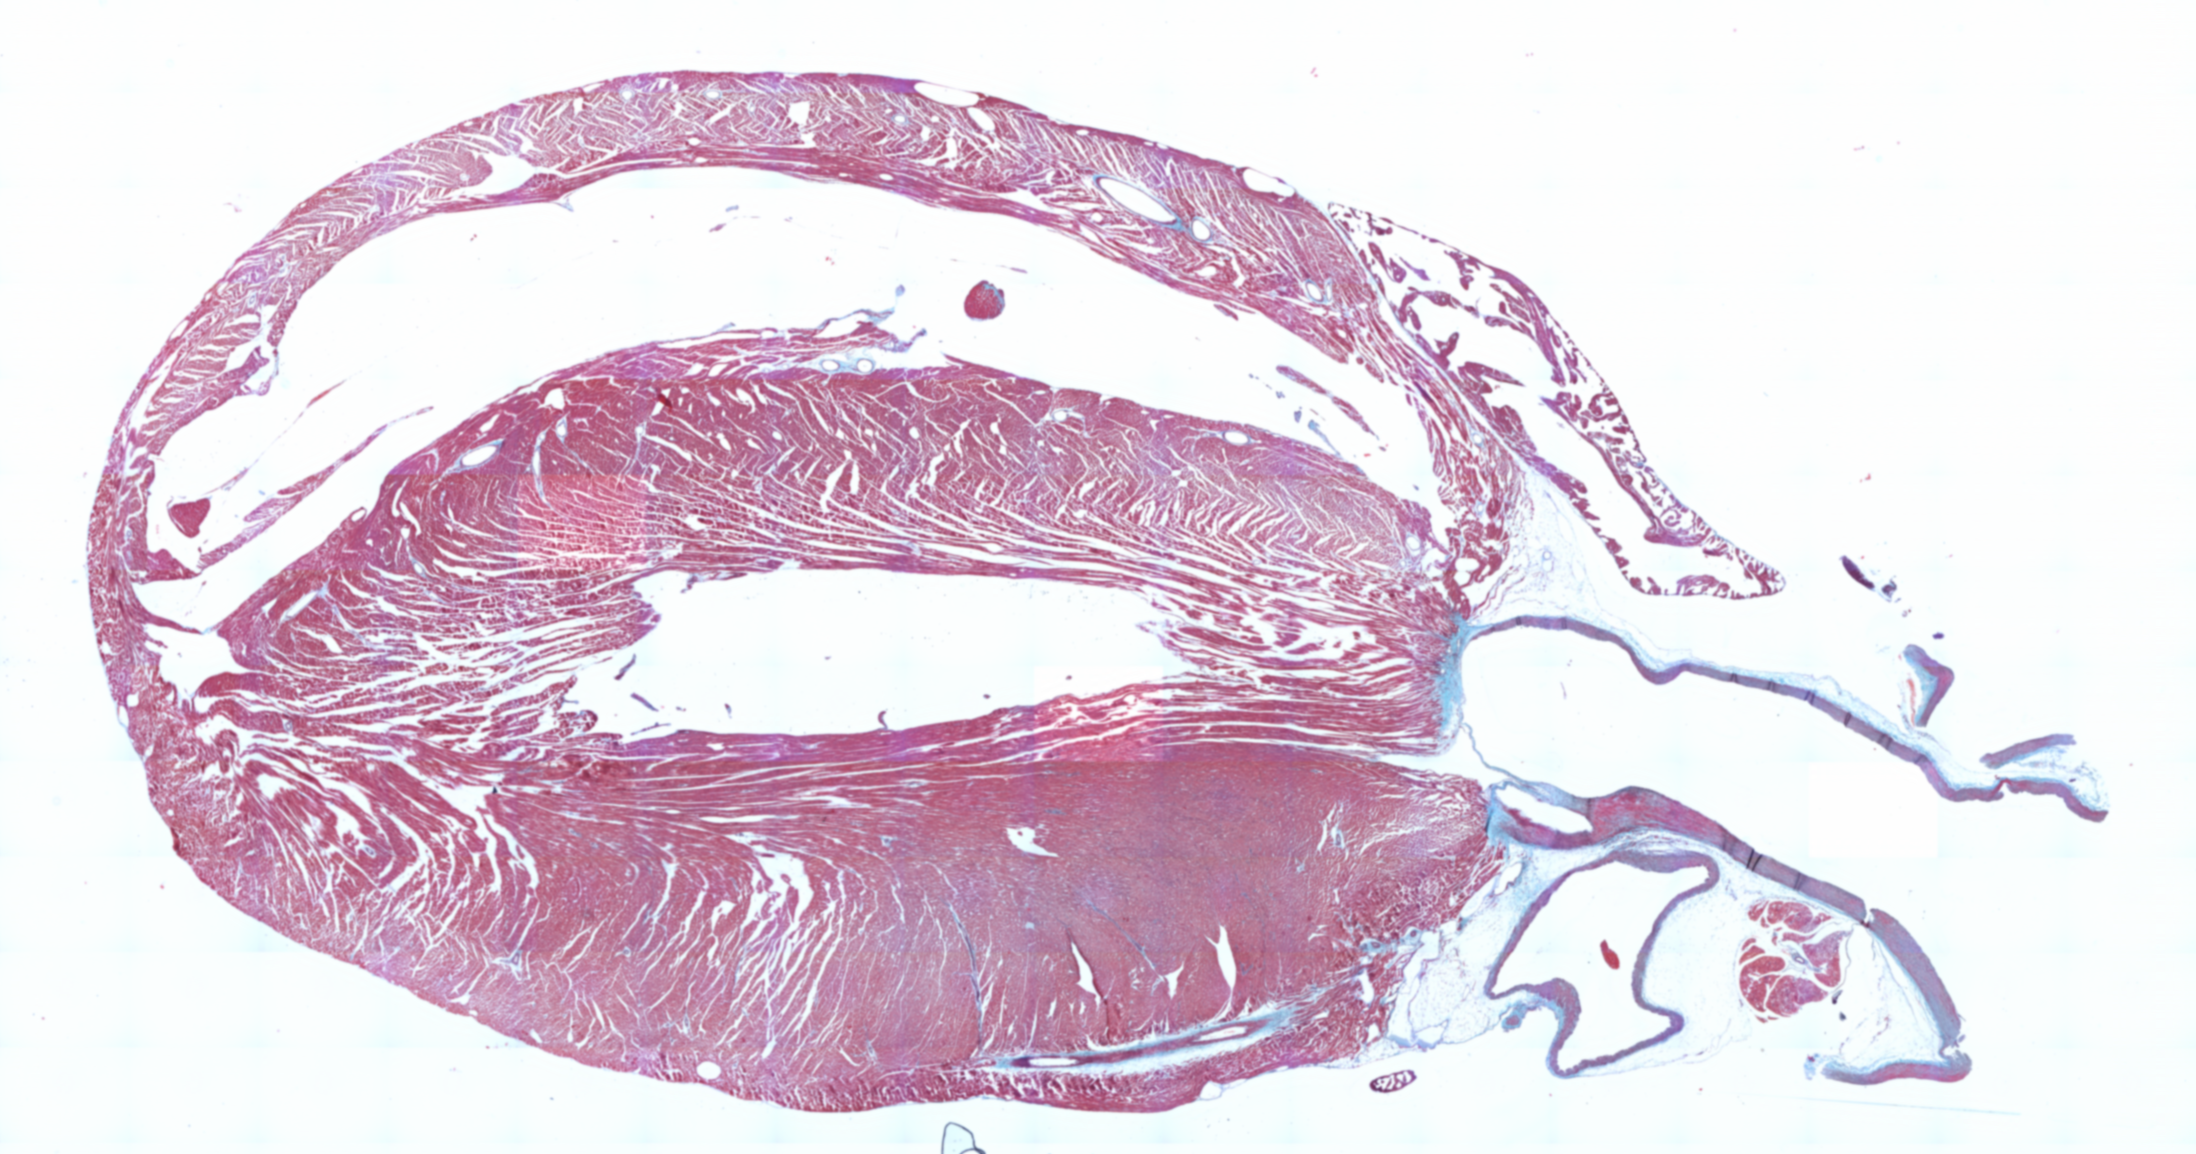
\includegraphics[width=1.7in]{1_motivation_and_aims/Figs/HiRes_downsamples_8_0582}}
    \subfloat[]{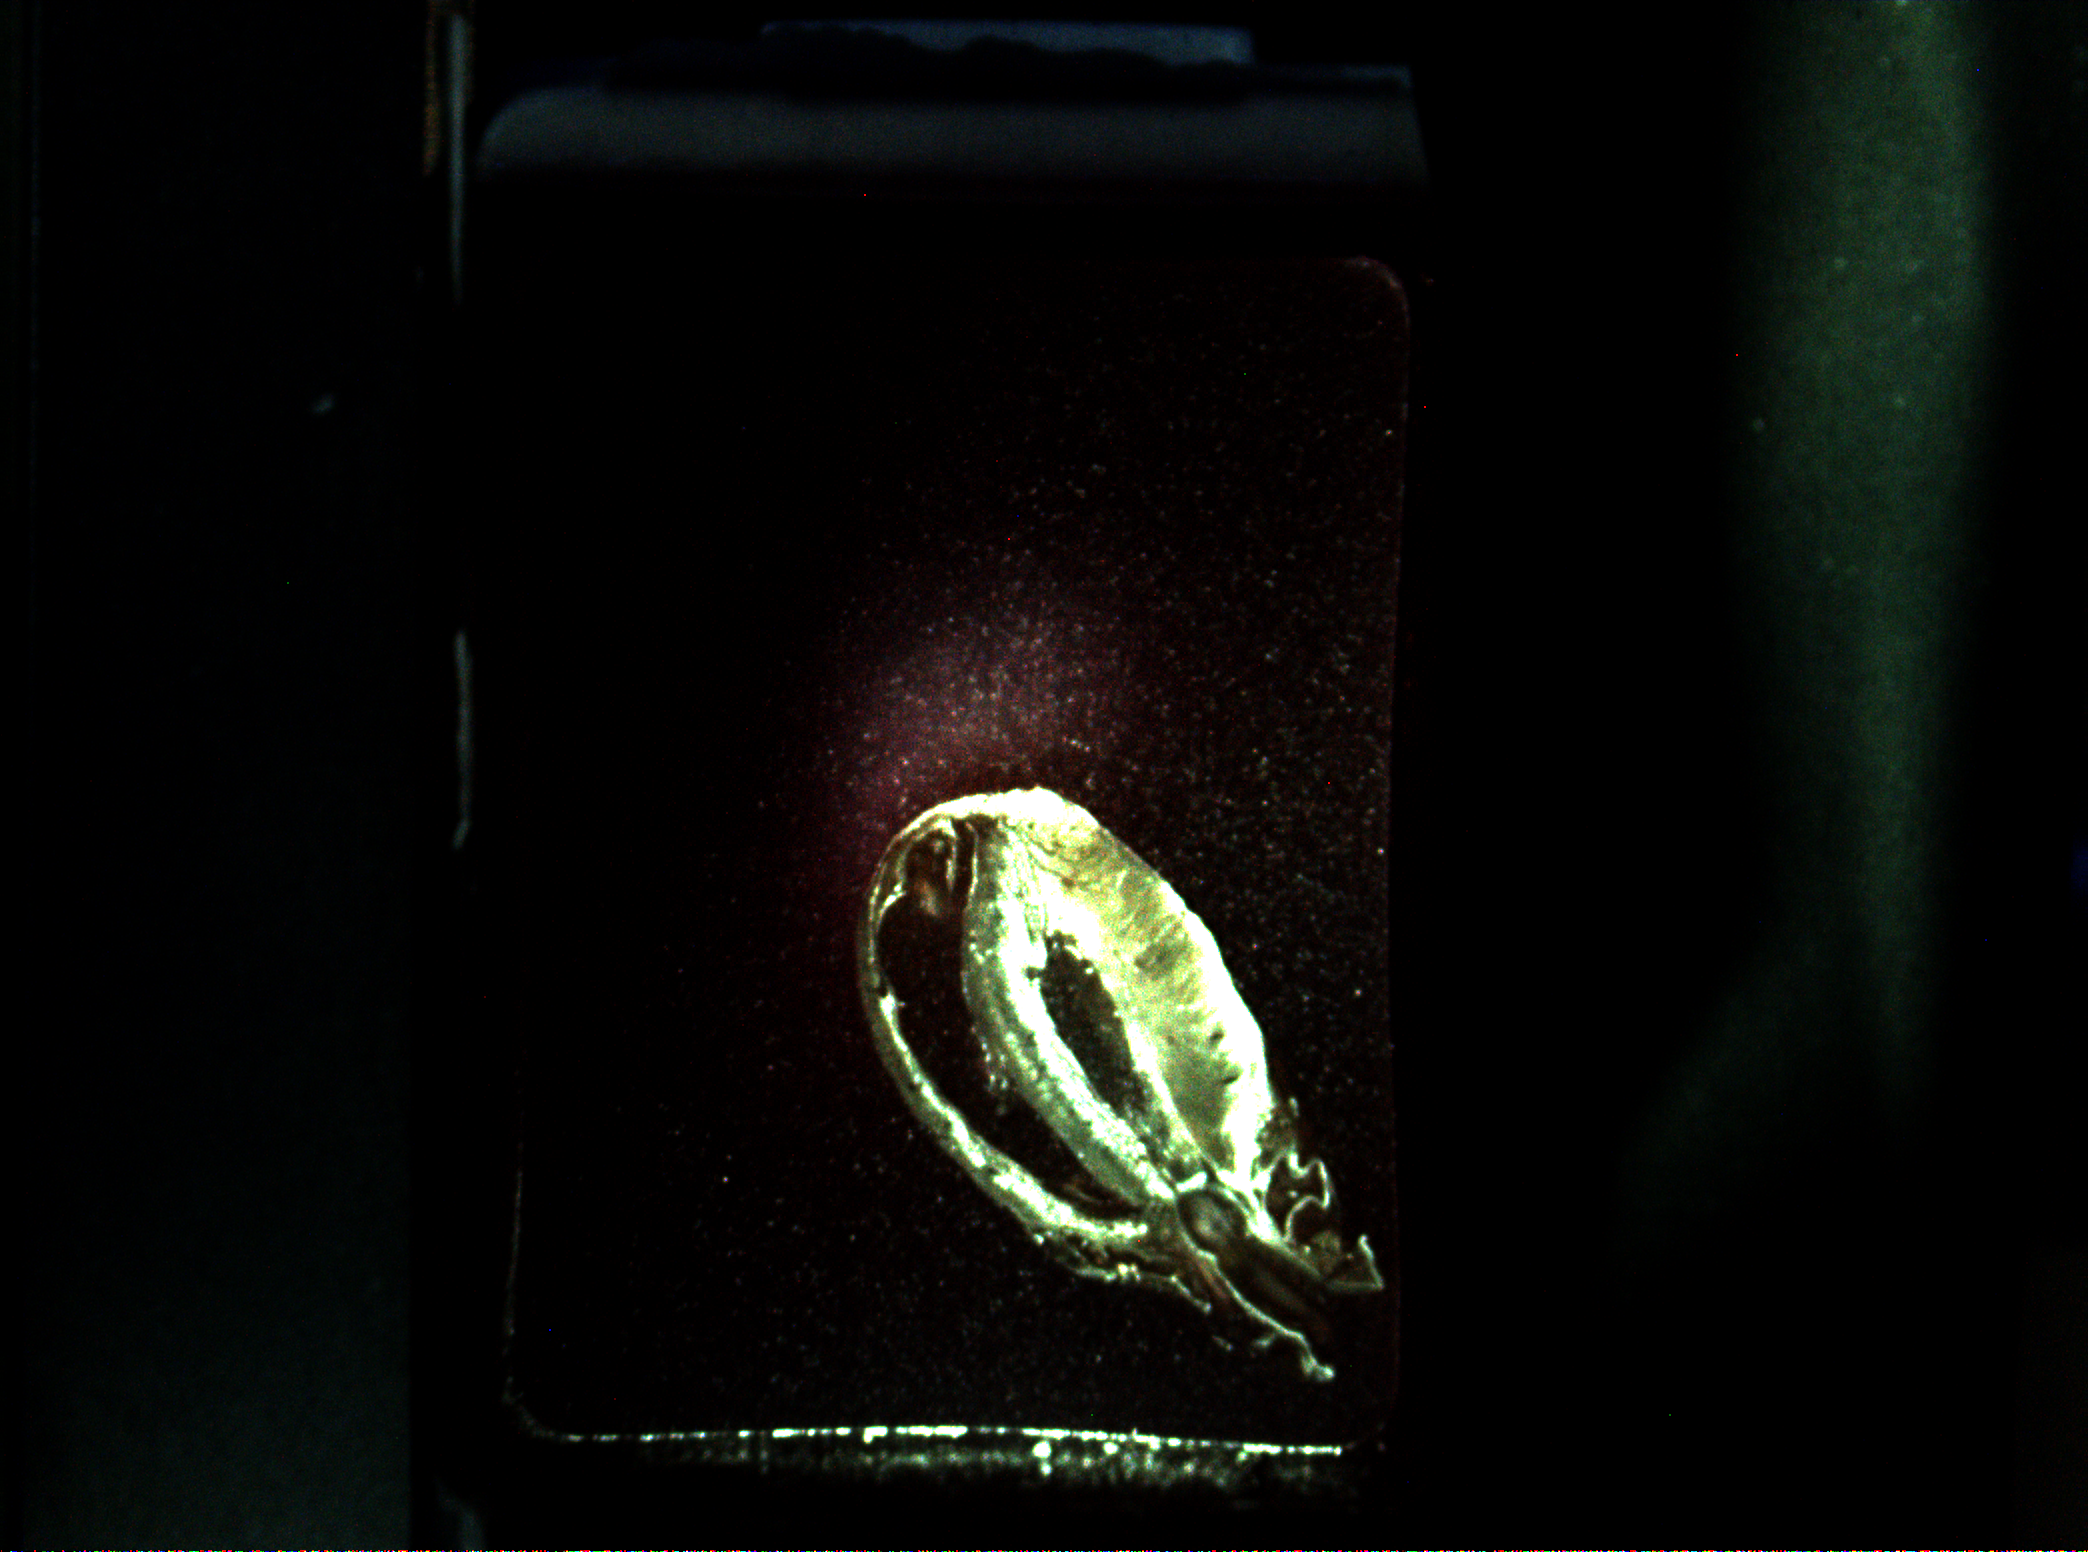
\includegraphics[width=1.7in]{1_motivation_and_aims/Figs/LoRes_rgb_downsamples_1_0582}}\\
    \subfloat[]{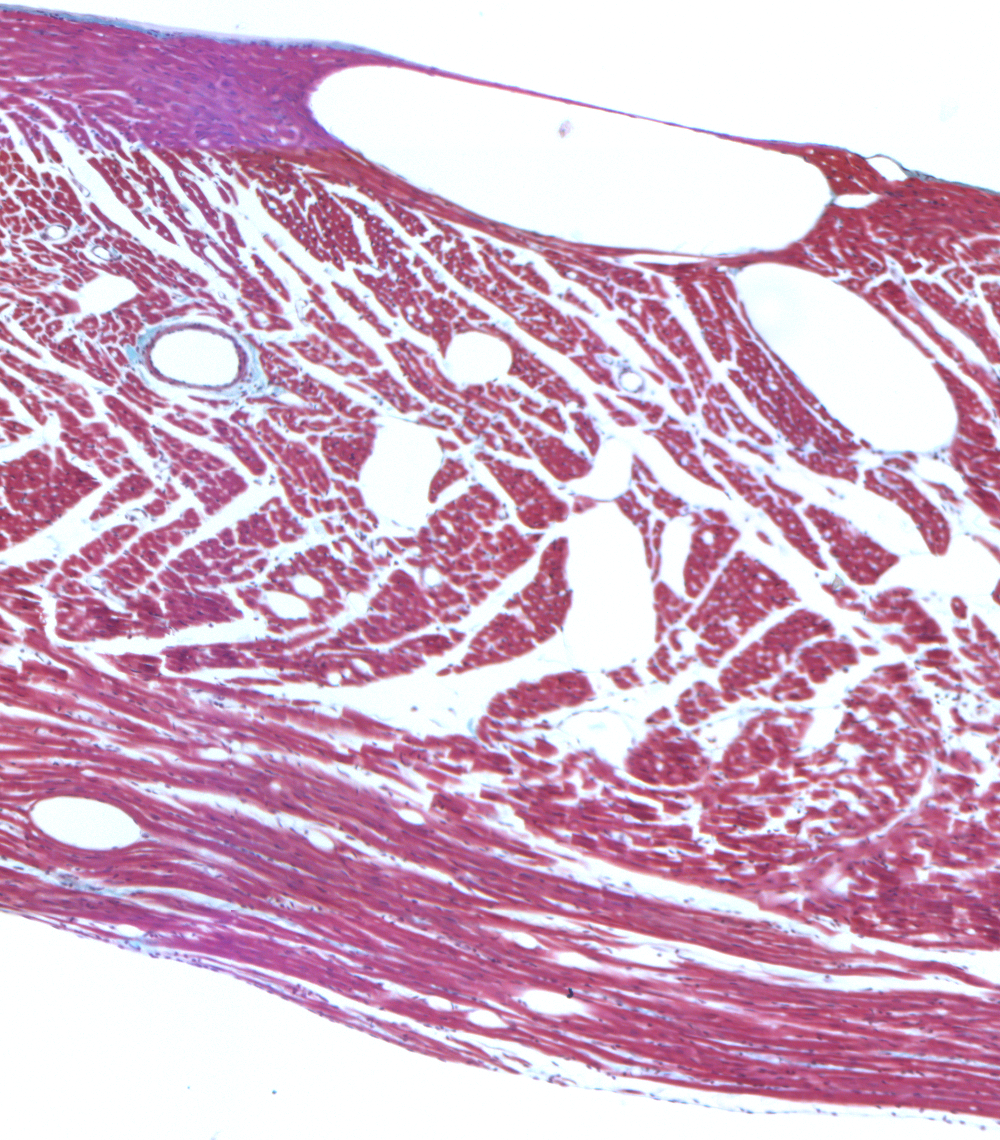
\includegraphics[width=1.7in]{1_motivation_and_aims/Figs/HiRes_downsamples_1_0582_zoom}}
    \subfloat[]{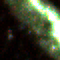
\includegraphics[width=1.7in]{1_motivation_and_aims/Figs/LoRes_rgb_downsamples_1_0582_zoom}}
    \caption{Figure on starting point, showing dataset images, whole and with zoom}
    \label{fig:synthetic_cross_sections}
  \end{figure}
    
  
% section motivation_and_aims (end)
